% E.14 正方形 ABCD 边长 4. E 在 AB 上. △ADE 沿 DE 折, A→A'.
% A(0,4), B(4,4), C(4,0), D(0,0). E=AB 中点 (2,4). AE=2.
% A 关于 DE 镜像: DE: 从 D(0,0) 到 E(2,4). DA=4 → DA'=4. ∠ADE = ∠EDA'.
% A'=镜像(A, DE). DE方向 (2,4)/√20=(1/√5, 2/√5). A=(0,4).
% 投影 A 到 DE: t=(A·d)/|d|² = (0·2+4·4)/20=0.8 → 足点 (1.6, 3.2). A' = 2·(1.6,3.2)-(0,4)=(3.2, 2.4).
\documentclass[tikz,border=4pt]{standalone}
\usepackage{ctex}
\usepackage{amsmath}
\usetikzlibrary{calc}
\begin{document}
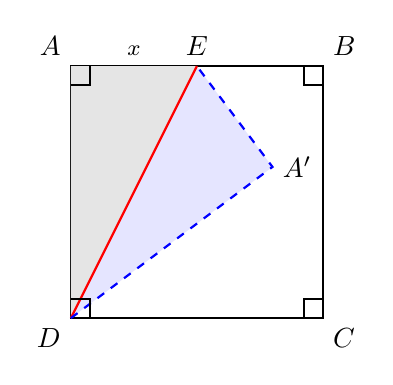
\begin{tikzpicture}[scale=0.8, thick]
  \coordinate (A) at (0,4);
  \coordinate (B) at (4,4);
  \coordinate (C) at (4,0);
  \coordinate (D) at (0,0);
  \coordinate (E) at (2,4);
  \coordinate (Ap) at (3.2, 2.4);

  \draw (A)--(B)--(C)--(D)--cycle;
  \fill[black!10] (A)--(D)--(E)--cycle;
  \fill[blue!10] (Ap)--(D)--(E)--cycle;
  \draw[red, thick] (D)--(E);
  \draw[blue, dashed, thick] (D)--(Ap)--(E);

  % 直角四个角
  \draw ($(A)+(0.3,0)$)--($(A)+(0.3,-0.3)$)--($(A)+(0,-0.3)$);
  \draw ($(B)+(-0.3,0)$)--($(B)+(-0.3,-0.3)$)--($(B)+(0,-0.3)$);
  \draw ($(C)+(-0.3,0)$)--($(C)+(-0.3,0.3)$)--($(C)+(0,0.3)$);
  \draw ($(D)+(0.3,0)$)--($(D)+(0.3,0.3)$)--($(D)+(0,0.3)$);

  \node[above left] at (A) {$A$};
  \node[above right] at (B) {$B$};
  \node[below right] at (C) {$C$};
  \node[below left] at (D) {$D$};
  \node[above] at (E) {$E$};
  \node[right] at (Ap) {$A'$};

  \node[font=\footnotesize, above] at ($(A)!0.5!(E)$) {$x$};
\end{tikzpicture}
\end{document}
